Models of bottom-flavored Dark Matter that are closely related to the \tchannel mediated model from this 
Section have been proposed in Refs.~\cite{Lin:2013sca,Agrawal:2014una}. 
Here, DM couples preferentially to bottom quarks, with a decoupled third generation. 
We describe the $b$-FDM model of Ref.~\cite{Agrawal:2014una}, created to explain the Galactic Center (GC) 
gamma-ray excess observed in data collected by the Fermi-LAT collaboration~\cite{Daylan:2014rsa,Calore:2014xka}. 
This model favors couplings to third-generation quarks via Yukawa couplings, 
therefore respecting the MFV assumption. 

This model produces an annihilation cross section consistent with the gamma-ray excess
which can be achieved for perturbative
values of the couplings, while being consistent with LHC constraints on the
colored mediator
For parameters capable of explaining the anomalous gamma-ray signal in terms of Dark Matter 
coupling preferentially to $b$-quarks, the model predicts a direct detection cross section that is consistent 
with current constraints, but within the near future reach of Direct Detection experiments and of the
upcoming LHC run. 
%The model will be decisively tested with data from the upcoming high-energy run at the LHC. 

The model contains a Dirac fermion transforming as a flavor triplet, exclusively coupling
to right-handed down-type quarks. The third component of the triplet $\chi_b$ comprises the 
cosmological DM. Within the MFV framework, the other fermions in the flavor triplet can be 
made sufficiently heavy and weakly-coupled that they can be neglected in the analysis.
A flavor singlet, color triplet scalar field $\Phi$ mediates the interactions between the DM 
and the Standard Model quarks.  The model is similar to the MSSM with a light bottom squark and neutralino, 
and is thus a flavor-specific example of a \tchannel model. 
Similar top-flavored models can exist, as e.g. in Refs.~\cite{Kumar:2013hfa,Batell:2013zwa}. 
In the case where the top coupling is the main DM coupling, 
the signal is very similar to a signal from a stop quark, since unlike the other t-channel cases there is no top
in the initial state PDFs. This is the reason why it wasn't considered as an additional model. More recent
literature shows that other flavor states could also contribute to LHC signals, as shown in Ref.~\cite{Kilic:2015vka},
but such models will have to be investigate on a longer timescale with respect to that of this Forum. 

The Lagrangian considered is given by
\begin{equation}
  -{\cal L} \supset g \Phi^* \bar\chi_b b_R  + {\rm h.c.}
\end{equation}

%The QCD production of the colored mediator introduces a tree-level $b$+MET diagram with a $g_s*g$ dependence, which could be scaled. 
%However, the bb+MET (which often also falls in the b+MET signal region) has both pure QCD production of the colored mediator 
%($g_s^2$) and also possibly diagrams that scale as $g_s^2*g$. 

\paragraph{Parameter scan}

The nature of the model is not conducive to a simple scaling behavior that would allow us to reduce the number of points to be simulated. This is because of the interference of diagrams with QCD production of the mediator (which scale as $g^2_s$) with diagrams that are proportional to the coupling $g$ in the $b+$\MET{} and $b\bar{b}$+\MET{} final states. Fixing the couplings also fixes the mediator width, when adopting the minimal width assumption. 

A full study of the parameter scan for this model was not available for this report; thus we recommend scanning a range of  possible widths as discussed in a more-limited way for the \schannel mono-jet, spanning from the minimal width to a value approaching the particle limit, e.g. $g=0.5,1,2,3$. A coupling benchmark such as $g=1$ should be considered for each mass point since this would be a distinctive feature of this benchmark from SUSY models with sbottom squarks (see Section~\ref{sec:monojet_t_channel} for further discussion).
%: Cross-sections for unit couplings can be found in Appendix~\ref{app:xsecs_bFDM}. 
%The coupling could also be chosen to fulfill constraints from the relic density (see Appendix~\ref{app:Relic_Density_bFDM}, with corresponding cross sections in Tables~\ref{tab:g_relic_13T} onwards). 

A scan of Dark Matter and mediator masses should be done in the on-shell region $\MPhi > \mDM + m_b$, since the cross-sections in the off-shell region are too small to be probed with early LHC data, spanning from 10 to 500 GeV in \mDM and from 10 to 1300 GeV in \MPhi. 

%  \item $\mDM=10-500$ GeV with a binning of 50 GeV for $\mDM<100$ and  100 GeV otherwise; 
%  \item $\MPhi=10-1300$ with a binning of 100 GeV;

% Therefore, the coupling scan is chosen as a discrete set of values $g=0.5,1,2,3$ for each mass point.
%~\Todo{Are we sure the models in SVN have minimal width? What is the max coupling so that the width is still lower than the mass?}

\begin{figure*}[h!]
  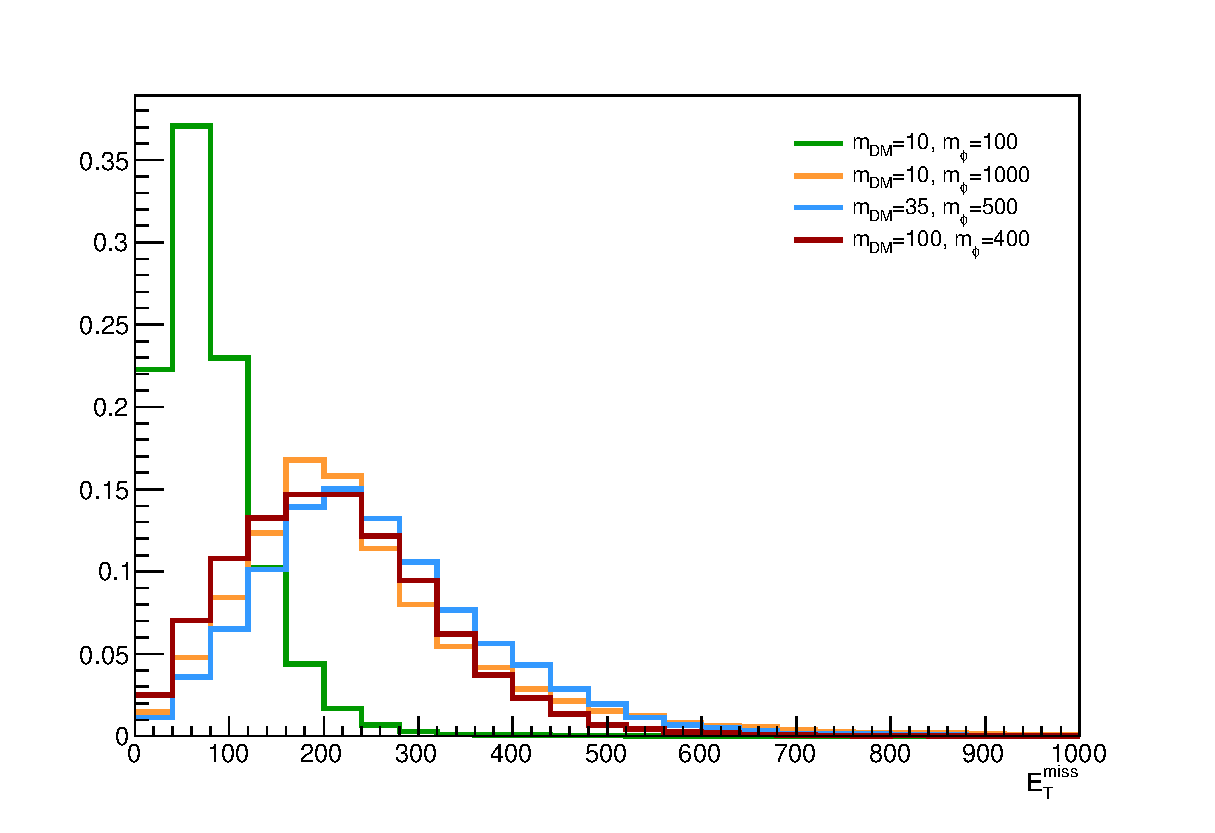
\includegraphics[width=0.49\textwidth]{figures/bFDM/bfdm_relic/missing_et.eps}\quad
  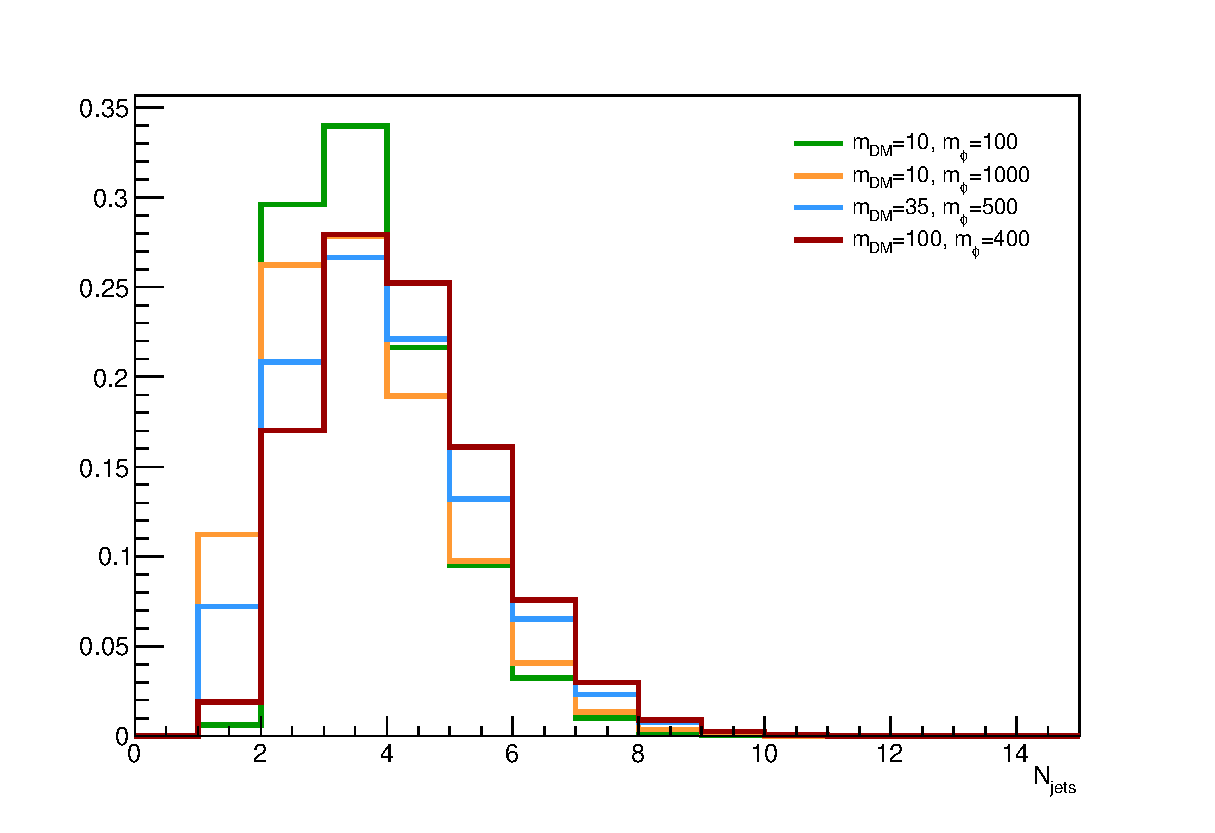
\includegraphics[width=0.49\textwidth]{figures/bFDM/bfdm_relic/Njets.eps}
  \caption{\MET (left) and jet multiplicity (right) for various DM and mediator masses and couplings normalized to the relic density observed in the early universe.}\label{fig:relic}
\end{figure*}

\begin{figure*}[h!]
  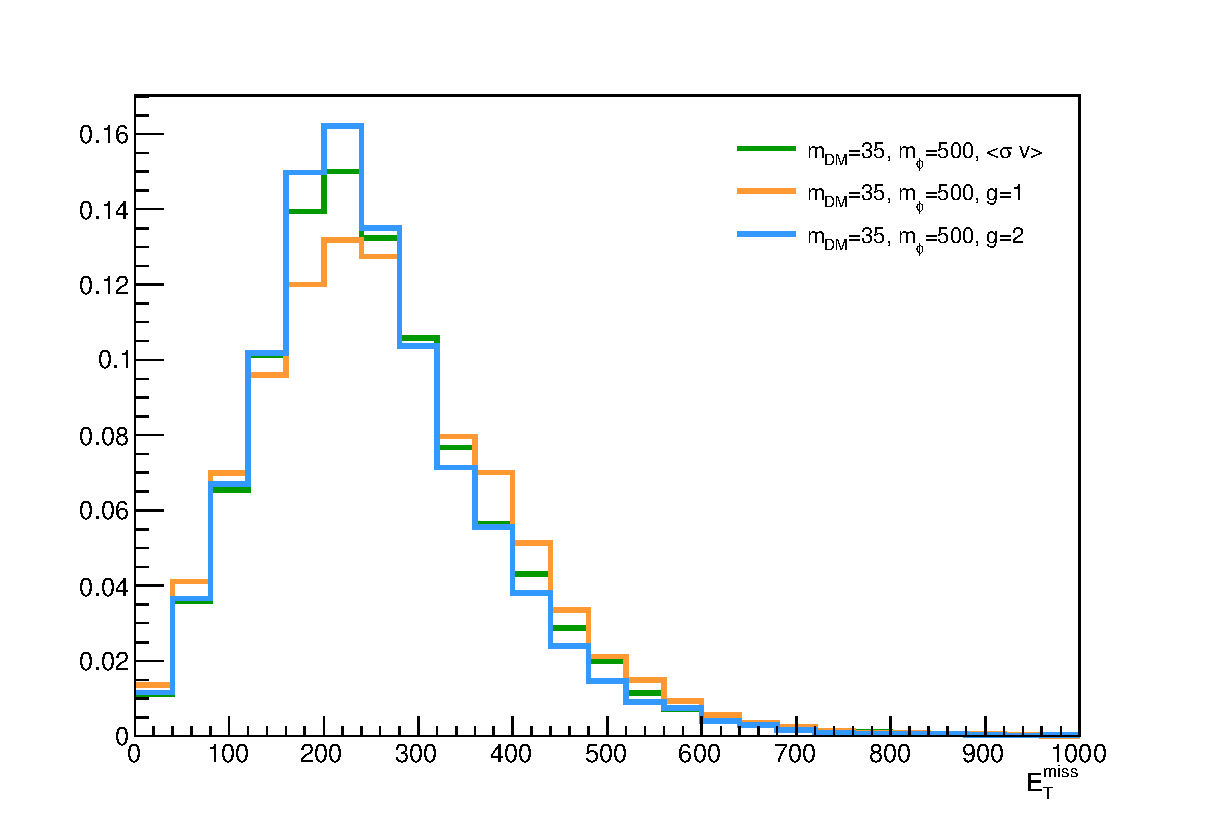
\includegraphics[width=0.49\textwidth]{figures/bFDM/bfdm_35_500/missing_et.eps}\quad
  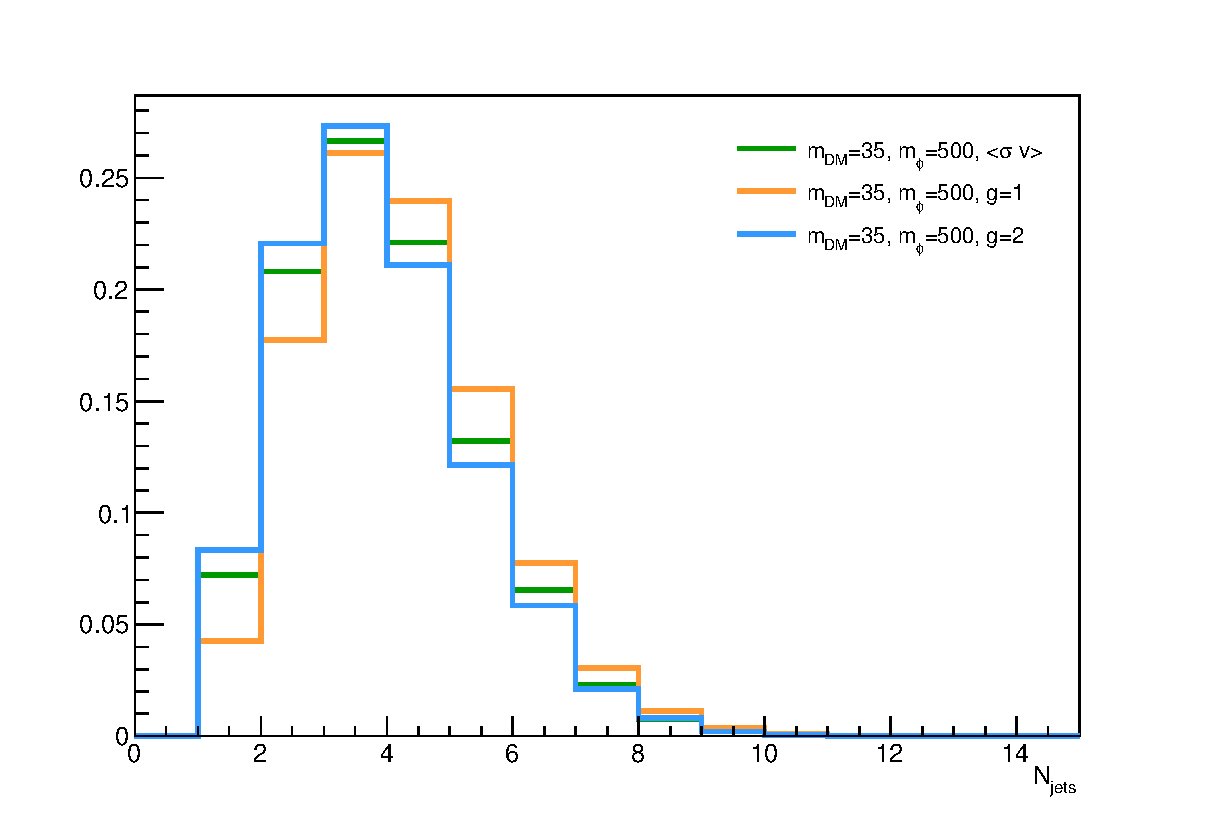
\includegraphics[width=0.49\textwidth]{figures/bFDM/bfdm_35_500/Njets.eps}
  \caption{\MET (left) and jet multiplicity (right) for $\mDM=35$~GeV and $\MPhi=500$~GeV for couplings corresponding to relic density weights and also $g=1,2$} \label{fig:g_comp}
\end{figure*}

%The following benchmark points could be produced as a starting point for the parameter space for this model:
%
%\begin{itemize}
%  \item $\mDM=10-500$ GeV with a binning of 50 GeV for $\mDM<100$ and  100 GeV otherwise; 
%  \item $\MPhi=10-1300$ with a binning of 100 GeV;
%  \item $\MPhi > \mDM + m_b$, since the cross-sections in the off-shell region are too small to be sensitive with early LHC data;
%\end{itemize}

%This scan of the parameter space is summarized in Table~\ref{tab:monobscan}.
%
%\begin{table}[!h]
%\centering
%\resizebox{\textwidth}{!}{
%\begin{tabular}{| l |r r r r r r r r r r r r r r|}
%\hline
%\multicolumn{1}{|c|}{\mDM (\gev)} & \multicolumn{14}{c|}{\mmed (\gev)} \\
%\hline
%  10 &   10 &  100 &  200 &  300 &  400 &  500 &  600 &  700 &  800 &  900 & 1000 & 1100 & 1200 & 1300 \\
%  50 &      &  100 &  200 &  300 &  400 &  500 &  600 &  700 &  800 &  900 & 1000 & 1100 & 1200 & 1300 \\
% 100 &      &  100 &  200 &  300 &  400 &  500 &  600 &  700 &  800 &  900 & 1000 & 1100 & 1200 & 1300 \\
% 200 &      &      &  200 &  300 &  400 &  500 &  600 &  700 &  800 &  900 & 1000 & 1100 & 1200 & 1300 \\
% 300 &      &      &      &  300 &  400 &  500 &  600 &  700 &  800 &  900 & 1000 & 1100 & 1200 & 1300 \\
% 400 &      &      &      &      &  400 &  500 &  600 &  700 &  800 &  900 & 1000 & 1100 & 1200 & 1300 \\
% 500 &      &      &      &      &      &  500 &  600 &  700 &  800 &  900 & 1000 & 1100 & 1200 & 1300 \\
%\hline
%\end{tabular}
%}
%\caption{Simplified model benchmarks for the considered mono-$b$ model, as described in the text.}
%\label{tab:monobscan}
%\end{table}

%The increase in the center of mass energy from 8 to 13 TeV leads to a cross-section increase that is a function of \MPhi, 
%with a smaller dependency for \mDM. Therefore, the sensitivity to this model will increase in early 13~TeV data compared to 8 TeV searches~\cite{Aad:2014vea}.

